\section{Introduction}
This section describes the various options available to the users for instantiating and
parametrising the WRPC in their designs.

\begin{figure}
  \begin{center}
    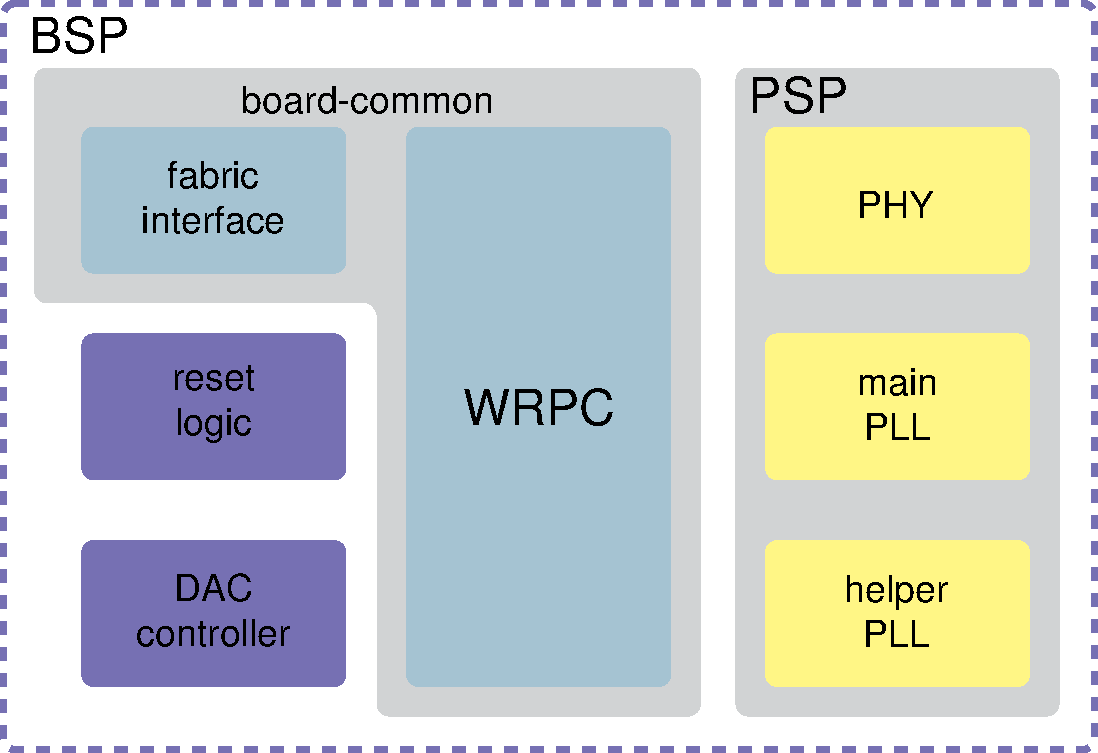
\includegraphics[width=.6\textwidth]{fig/wrpc_board.pdf}
    \label{fig:wrpc_board}
    \caption{WRPC HDL abstraction hierarchy}
  \end{center}
\end{figure}

The WRPC provides several levels of abstractions and VHDL modules, depending on the target
system. These are presented in Figure~\ref{fig:wrpc_board}. At the highest level of abstraction, the
WRPC provides Board Support Packages (BSPs), available for all officially supported boards. All BSP
modules share a common part (the ``board-common'' module) which encapsulates the WRPC core itself,
together with a selection of interfaces for connecting the core the the user FPGA
logic. Furthermore, each BSP also makes use of a Platform Support Package (PSP), which groups
together and instantiates all the FPGA-specific parts (typically hard IP provided by the FPGA
vendor), such as PHY, PLLs and clock buffers.

Thus, depending on the users' systems and needs, several scenarios might be available for
instantiating the WRPC into their designs.

\begin{description}
  \item[Option 1: Supported board.] In this simplest of scenarios, it will be enough to just
    instantiate the provided BSP into the users' designs and configure it via the provided generics.
  \item[Option 2: Supported FPGA platform.] The users could draw inspiration from an existing BSP
    based on the same platform, reusing the board-common module and PSP, while adapting the parts
    that are unique to their designs.
  \item[Option 3: Unsupported FPGA platform.] There is significant work involved in this
    scenario. In addition to providing the details for their board (just like for option 2), users
    also have to write their own PSP. It should be possible though to reuse the board-common
    module. Furthermore, if the unsupported platform is related to a supported one, it could be that
    the PHY and/or PLLs will also be reused, perhaps with minor adjustments.
\end{description}

When writing a new BSP or PSP, it's worth discussing it first in the
\href{http://www.ohwr.org/mailing_list/show?project_id=white-rabbit}{white-rabbit-dev} mailing
list. Perhaps there is already some preliminary support underway. It's also worth considering
sharing your work so that it can be merged with the project and added to the list of supported
platforms/boards.

The rest of this section describes the various modules in more detail. The WRPC module is presented
in Section~\ref{sec:hdl_wrpc}. The platform support modules are presented in
Section~\ref{sec:hdl_platform}, while the board support modules are presented in
Section~\ref{sec:hdl_board}.

